% Created by tikzDevice version 0.12.6 on 2026-02-22 21:41:52
% !TEX encoding = UTF-8 Unicode
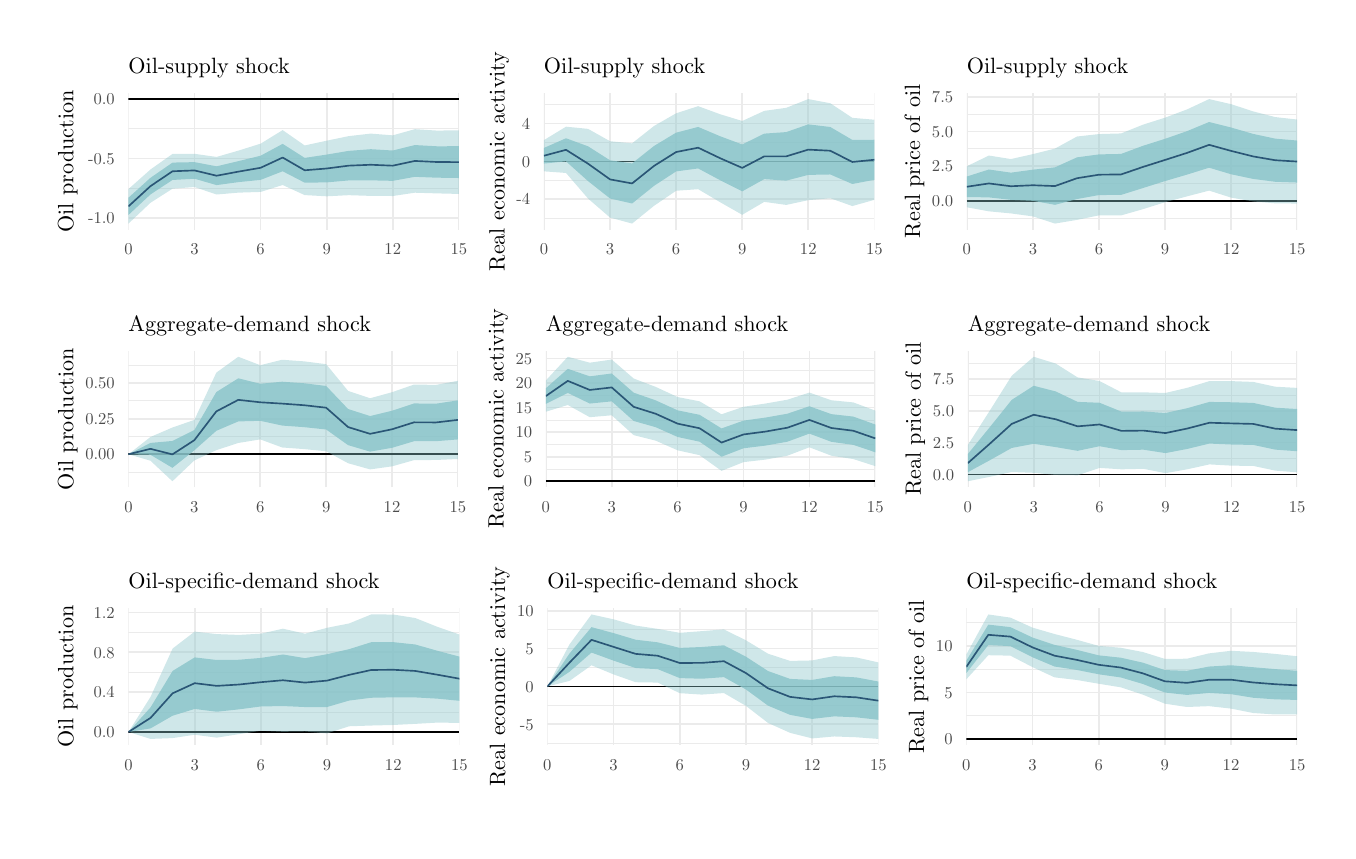
\begin{tikzpicture}[x=1pt,y=1pt]
\definecolor{fillColor}{RGB}{255,255,255}
\path[use as bounding box,fill=fillColor,fill opacity=0.00] (0,0) rectangle (469.75,290.32);
\begin{scope}
\path[clip] ( 36.43,217.28) rectangle (155.81,266.76);
\definecolor{drawColor}{gray}{0.92}

\path[draw=drawColor,line width= 0.3pt,line join=round] ( 36.43,232.29) --
	(155.81,232.29);

\path[draw=drawColor,line width= 0.3pt,line join=round] ( 36.43,253.77) --
	(155.81,253.77);

\path[draw=drawColor,line width= 0.6pt,line join=round] ( 36.43,221.55) --
	(155.81,221.55);

\path[draw=drawColor,line width= 0.6pt,line join=round] ( 36.43,243.03) --
	(155.81,243.03);

\path[draw=drawColor,line width= 0.6pt,line join=round] ( 36.43,264.51) --
	(155.81,264.51);

\path[draw=drawColor,line width= 0.6pt,line join=round] ( 36.43,217.28) --
	( 36.43,266.76);

\path[draw=drawColor,line width= 0.6pt,line join=round] ( 60.30,217.28) --
	( 60.30,266.76);

\path[draw=drawColor,line width= 0.6pt,line join=round] ( 84.18,217.28) --
	( 84.18,266.76);

\path[draw=drawColor,line width= 0.6pt,line join=round] (108.06,217.28) --
	(108.06,266.76);

\path[draw=drawColor,line width= 0.6pt,line join=round] (131.93,217.28) --
	(131.93,266.76);

\path[draw=drawColor,line width= 0.6pt,line join=round] (155.81,217.28) --
	(155.81,266.76);
\definecolor{drawColor}{RGB}{0,0,0}

\path[draw=drawColor,line width= 0.6pt,line join=round] ( 36.43,264.51) -- (155.81,264.51);
\definecolor{fillColor}{RGB}{136,195,200}

\path[fill=fillColor,fill opacity=0.40] ( 36.43,232.01) --
	( 44.39,239.08) --
	( 52.35,244.71) --
	( 60.30,244.73) --
	( 68.26,243.61) --
	( 76.22,245.91) --
	( 84.18,248.41) --
	( 92.14,253.30) --
	(100.10,247.76) --
	(108.06,249.48) --
	(116.01,251.13) --
	(123.97,252.04) --
	(131.93,251.41) --
	(139.89,253.64) --
	(147.85,253.13) --
	(155.81,253.23) --
	(155.81,230.24) --
	(147.85,230.44) --
	(139.89,230.68) --
	(131.93,229.49) --
	(123.97,229.53) --
	(116.01,229.79) --
	(108.06,229.38) --
	(100.10,229.82) --
	( 92.14,233.47) --
	( 84.18,230.96) --
	( 76.22,230.71) --
	( 68.26,230.03) --
	( 60.30,232.73) --
	( 52.35,232.14) --
	( 44.39,227.06) --
	( 36.43,219.53) --
	cycle;

\path[] ( 36.43,232.01) --
	( 44.39,239.08) --
	( 52.35,244.71) --
	( 60.30,244.73) --
	( 68.26,243.61) --
	( 76.22,245.91) --
	( 84.18,248.41) --
	( 92.14,253.30) --
	(100.10,247.76) --
	(108.06,249.48) --
	(116.01,251.13) --
	(123.97,252.04) --
	(131.93,251.41) --
	(139.89,253.64) --
	(147.85,253.13) --
	(155.81,253.23);

\path[] (155.81,230.24) --
	(147.85,230.44) --
	(139.89,230.68) --
	(131.93,229.49) --
	(123.97,229.53) --
	(116.01,229.79) --
	(108.06,229.38) --
	(100.10,229.82) --
	( 92.14,233.47) --
	( 84.18,230.96) --
	( 76.22,230.71) --
	( 68.26,230.03) --
	( 60.30,232.73) --
	( 52.35,232.14) --
	( 44.39,227.06) --
	( 36.43,219.53);
\definecolor{fillColor}{RGB}{136,195,200}

\path[fill=fillColor,fill opacity=0.80] ( 36.43,228.89) --
	( 44.39,236.08) --
	( 52.35,241.57) --
	( 60.30,241.73) --
	( 68.26,240.22) --
	( 76.22,242.11) --
	( 84.18,244.05) --
	( 92.14,248.34) --
	(100.10,243.27) --
	(108.06,244.46) --
	(116.01,245.80) --
	(123.97,246.41) --
	(131.93,245.93) --
	(139.89,247.90) --
	(147.85,247.46) --
	(155.81,247.48) --
	(155.81,235.99) --
	(147.85,236.11) --
	(139.89,236.42) --
	(131.93,234.97) --
	(123.97,235.15) --
	(116.01,235.12) --
	(108.06,234.41) --
	(100.10,234.31) --
	( 92.14,238.43) --
	( 84.18,235.32) --
	( 76.22,234.51) --
	( 68.26,233.43) --
	( 60.30,235.73) --
	( 52.35,235.29) --
	( 44.39,230.07) --
	( 36.43,222.65) --
	cycle;

\path[] ( 36.43,228.89) --
	( 44.39,236.08) --
	( 52.35,241.57) --
	( 60.30,241.73) --
	( 68.26,240.22) --
	( 76.22,242.11) --
	( 84.18,244.05) --
	( 92.14,248.34) --
	(100.10,243.27) --
	(108.06,244.46) --
	(116.01,245.80) --
	(123.97,246.41) --
	(131.93,245.93) --
	(139.89,247.90) --
	(147.85,247.46) --
	(155.81,247.48);

\path[] (155.81,235.99) --
	(147.85,236.11) --
	(139.89,236.42) --
	(131.93,234.97) --
	(123.97,235.15) --
	(116.01,235.12) --
	(108.06,234.41) --
	(100.10,234.31) --
	( 92.14,238.43) --
	( 84.18,235.32) --
	( 76.22,234.51) --
	( 68.26,233.43) --
	( 60.30,235.73) --
	( 52.35,235.29) --
	( 44.39,230.07) --
	( 36.43,222.65);
\definecolor{drawColor}{RGB}{42,86,118}

\path[draw=drawColor,line width= 0.6pt,line join=round] ( 36.43,225.77) --
	( 44.39,233.07) --
	( 52.35,238.43) --
	( 60.30,238.73) --
	( 68.26,236.82) --
	( 76.22,238.31) --
	( 84.18,239.69) --
	( 92.14,243.39) --
	(100.10,238.79) --
	(108.06,239.43) --
	(116.01,240.46) --
	(123.97,240.78) --
	(131.93,240.45) --
	(139.89,242.16) --
	(147.85,241.78) --
	(155.81,241.73);
\end{scope}
\begin{scope}
\path[clip] (  0.00,  0.00) rectangle (469.75,290.32);
\definecolor{drawColor}{gray}{0.30}

\node[text=drawColor,anchor=base east,inner sep=0pt, outer sep=0pt, scale=  0.60] at ( 31.48,219.49) {-1.0};

\node[text=drawColor,anchor=base east,inner sep=0pt, outer sep=0pt, scale=  0.60] at ( 31.48,240.97) {-0.5};

\node[text=drawColor,anchor=base east,inner sep=0pt, outer sep=0pt, scale=  0.60] at ( 31.48,262.44) {0.0};
\end{scope}
\begin{scope}
\path[clip] (  0.00,  0.00) rectangle (469.75,290.32);
\definecolor{drawColor}{gray}{0.30}

\node[text=drawColor,anchor=base,inner sep=0pt, outer sep=0pt, scale=  0.60] at ( 36.43,208.20) {0};

\node[text=drawColor,anchor=base,inner sep=0pt, outer sep=0pt, scale=  0.60] at ( 60.30,208.20) {3};

\node[text=drawColor,anchor=base,inner sep=0pt, outer sep=0pt, scale=  0.60] at ( 84.18,208.20) {6};

\node[text=drawColor,anchor=base,inner sep=0pt, outer sep=0pt, scale=  0.60] at (108.06,208.20) {9};

\node[text=drawColor,anchor=base,inner sep=0pt, outer sep=0pt, scale=  0.60] at (131.93,208.20) {12};

\node[text=drawColor,anchor=base,inner sep=0pt, outer sep=0pt, scale=  0.60] at (155.81,208.20) {15};
\end{scope}
\begin{scope}
\path[clip] (  0.00,  0.00) rectangle (469.75,290.32);
\definecolor{drawColor}{RGB}{0,0,0}

\node[text=drawColor,rotate= 90.00,anchor=base,inner sep=0pt, outer sep=0pt, scale=  0.80] at ( 16.51,242.02) {Oil production};
\end{scope}
\begin{scope}
\path[clip] (  0.00,  0.00) rectangle (469.75,290.32);
\definecolor{drawColor}{RGB}{0,0,0}

\node[text=drawColor,anchor=base west,inner sep=0pt, outer sep=0pt, scale=  0.80] at ( 36.43,273.81) {Oil-supply shock};
\end{scope}
\begin{scope}
\path[clip] (186.57,217.28) rectangle (305.95,266.76);
\definecolor{drawColor}{gray}{0.92}

\path[draw=drawColor,line width= 0.3pt,line join=round] (186.57,221.52) --
	(305.95,221.52);

\path[draw=drawColor,line width= 0.3pt,line join=round] (186.57,235.17) --
	(305.95,235.17);

\path[draw=drawColor,line width= 0.3pt,line join=round] (186.57,248.83) --
	(305.95,248.83);

\path[draw=drawColor,line width= 0.3pt,line join=round] (186.57,262.48) --
	(305.95,262.48);

\path[draw=drawColor,line width= 0.6pt,line join=round] (186.57,228.34) --
	(305.95,228.34);

\path[draw=drawColor,line width= 0.6pt,line join=round] (186.57,242.00) --
	(305.95,242.00);

\path[draw=drawColor,line width= 0.6pt,line join=round] (186.57,255.65) --
	(305.95,255.65);

\path[draw=drawColor,line width= 0.6pt,line join=round] (186.57,217.28) --
	(186.57,266.76);

\path[draw=drawColor,line width= 0.6pt,line join=round] (210.45,217.28) --
	(210.45,266.76);

\path[draw=drawColor,line width= 0.6pt,line join=round] (234.32,217.28) --
	(234.32,266.76);

\path[draw=drawColor,line width= 0.6pt,line join=round] (258.20,217.28) --
	(258.20,266.76);

\path[draw=drawColor,line width= 0.6pt,line join=round] (282.07,217.28) --
	(282.07,266.76);

\path[draw=drawColor,line width= 0.6pt,line join=round] (305.95,217.28) --
	(305.95,266.76);
\definecolor{drawColor}{RGB}{0,0,0}

\path[draw=drawColor,line width= 0.6pt,line join=round] (186.57,242.00) -- (305.95,242.00);
\definecolor{fillColor}{RGB}{136,195,200}

\path[fill=fillColor,fill opacity=0.40] (186.57,249.70) --
	(194.53,254.54) --
	(202.49,253.75) --
	(210.45,249.28) --
	(218.40,248.52) --
	(226.36,254.81) --
	(234.32,259.38) --
	(242.28,261.95) --
	(250.24,259.03) --
	(258.20,256.60) --
	(266.16,260.25) --
	(274.11,261.36) --
	(282.07,264.51) --
	(290.03,263.01) --
	(297.99,257.73) --
	(305.95,257.06) --
	(305.95,228.11) --
	(297.99,225.86) --
	(290.03,228.69) --
	(282.07,227.99) --
	(274.11,226.27) --
	(266.16,227.37) --
	(258.20,222.70) --
	(250.24,227.24) --
	(242.28,231.95) --
	(234.32,231.39) --
	(226.36,225.97) --
	(218.40,219.53) --
	(210.45,221.69) --
	(202.49,228.57) --
	(194.53,237.82) --
	(186.57,238.40) --
	cycle;

\path[] (186.57,249.70) --
	(194.53,254.54) --
	(202.49,253.75) --
	(210.45,249.28) --
	(218.40,248.52) --
	(226.36,254.81) --
	(234.32,259.38) --
	(242.28,261.95) --
	(250.24,259.03) --
	(258.20,256.60) --
	(266.16,260.25) --
	(274.11,261.36) --
	(282.07,264.51) --
	(290.03,263.01) --
	(297.99,257.73) --
	(305.95,257.06);

\path[] (305.95,228.11) --
	(297.99,225.86) --
	(290.03,228.69) --
	(282.07,227.99) --
	(274.11,226.27) --
	(266.16,227.37) --
	(258.20,222.70) --
	(250.24,227.24) --
	(242.28,231.95) --
	(234.32,231.39) --
	(226.36,225.97) --
	(218.40,219.53) --
	(210.45,221.69) --
	(202.49,228.57) --
	(194.53,237.82) --
	(186.57,238.40);
\definecolor{fillColor}{RGB}{136,195,200}

\path[fill=fillColor,fill opacity=0.80] (186.57,246.87) --
	(194.53,250.36) --
	(202.49,247.45) --
	(210.45,242.39) --
	(218.40,241.27) --
	(226.36,247.60) --
	(234.32,252.38) --
	(242.28,254.45) --
	(250.24,251.08) --
	(258.20,248.12) --
	(266.16,252.03) --
	(274.11,252.59) --
	(282.07,255.38) --
	(290.03,254.43) --
	(297.99,249.76) --
	(305.95,249.82) --
	(305.95,235.35) --
	(297.99,233.83) --
	(290.03,237.27) --
	(282.07,237.12) --
	(274.11,235.05) --
	(266.16,235.59) --
	(258.20,231.17) --
	(250.24,235.19) --
	(242.28,239.45) --
	(234.32,238.38) --
	(226.36,233.18) --
	(218.40,226.78) --
	(210.45,228.59) --
	(202.49,234.87) --
	(194.53,242.00) --
	(186.57,241.22) --
	cycle;

\path[] (186.57,246.87) --
	(194.53,250.36) --
	(202.49,247.45) --
	(210.45,242.39) --
	(218.40,241.27) --
	(226.36,247.60) --
	(234.32,252.38) --
	(242.28,254.45) --
	(250.24,251.08) --
	(258.20,248.12) --
	(266.16,252.03) --
	(274.11,252.59) --
	(282.07,255.38) --
	(290.03,254.43) --
	(297.99,249.76) --
	(305.95,249.82);

\path[] (305.95,235.35) --
	(297.99,233.83) --
	(290.03,237.27) --
	(282.07,237.12) --
	(274.11,235.05) --
	(266.16,235.59) --
	(258.20,231.17) --
	(250.24,235.19) --
	(242.28,239.45) --
	(234.32,238.38) --
	(226.36,233.18) --
	(218.40,226.78) --
	(210.45,228.59) --
	(202.49,234.87) --
	(194.53,242.00) --
	(186.57,241.22);
\definecolor{drawColor}{RGB}{42,86,118}

\path[draw=drawColor,line width= 0.6pt,line join=round] (186.57,244.05) --
	(194.53,246.18) --
	(202.49,241.16) --
	(210.45,235.49) --
	(218.40,234.03) --
	(226.36,240.39) --
	(234.32,245.38) --
	(242.28,246.95) --
	(250.24,243.14) --
	(258.20,239.65) --
	(266.16,243.81) --
	(274.11,243.82) --
	(282.07,246.25) --
	(290.03,245.85) --
	(297.99,241.79) --
	(305.95,242.59);
\end{scope}
\begin{scope}
\path[clip] (  0.00,  0.00) rectangle (469.75,290.32);
\definecolor{drawColor}{gray}{0.30}

\node[text=drawColor,anchor=base east,inner sep=0pt, outer sep=0pt, scale=  0.60] at (181.62,226.28) {-4};

\node[text=drawColor,anchor=base east,inner sep=0pt, outer sep=0pt, scale=  0.60] at (181.62,239.93) {0};

\node[text=drawColor,anchor=base east,inner sep=0pt, outer sep=0pt, scale=  0.60] at (181.62,253.59) {4};
\end{scope}
\begin{scope}
\path[clip] (  0.00,  0.00) rectangle (469.75,290.32);
\definecolor{drawColor}{gray}{0.30}

\node[text=drawColor,anchor=base,inner sep=0pt, outer sep=0pt, scale=  0.60] at (186.57,208.20) {0};

\node[text=drawColor,anchor=base,inner sep=0pt, outer sep=0pt, scale=  0.60] at (210.45,208.20) {3};

\node[text=drawColor,anchor=base,inner sep=0pt, outer sep=0pt, scale=  0.60] at (234.32,208.20) {6};

\node[text=drawColor,anchor=base,inner sep=0pt, outer sep=0pt, scale=  0.60] at (258.20,208.20) {9};

\node[text=drawColor,anchor=base,inner sep=0pt, outer sep=0pt, scale=  0.60] at (282.07,208.20) {12};

\node[text=drawColor,anchor=base,inner sep=0pt, outer sep=0pt, scale=  0.60] at (305.95,208.20) {15};
\end{scope}
\begin{scope}
\path[clip] (  0.00,  0.00) rectangle (469.75,290.32);
\definecolor{drawColor}{RGB}{0,0,0}

\node[text=drawColor,rotate= 90.00,anchor=base,inner sep=0pt, outer sep=0pt, scale=  0.80] at (172.32,242.02) {Real economic activity};
\end{scope}
\begin{scope}
\path[clip] (  0.00,  0.00) rectangle (469.75,290.32);
\definecolor{drawColor}{RGB}{0,0,0}

\node[text=drawColor,anchor=base west,inner sep=0pt, outer sep=0pt, scale=  0.80] at (186.57,273.81) {Oil-supply shock};
\end{scope}
\begin{scope}
\path[clip] (339.38,217.28) rectangle (458.75,266.76);
\definecolor{drawColor}{gray}{0.92}

\path[draw=drawColor,line width= 0.3pt,line join=round] (339.38,221.49) --
	(458.75,221.49);

\path[draw=drawColor,line width= 0.3pt,line join=round] (339.38,234.02) --
	(458.75,234.02);

\path[draw=drawColor,line width= 0.3pt,line join=round] (339.38,246.54) --
	(458.75,246.54);

\path[draw=drawColor,line width= 0.3pt,line join=round] (339.38,259.07) --
	(458.75,259.07);

\path[draw=drawColor,line width= 0.6pt,line join=round] (339.38,227.75) --
	(458.75,227.75);

\path[draw=drawColor,line width= 0.6pt,line join=round] (339.38,240.28) --
	(458.75,240.28);

\path[draw=drawColor,line width= 0.6pt,line join=round] (339.38,252.80) --
	(458.75,252.80);

\path[draw=drawColor,line width= 0.6pt,line join=round] (339.38,265.33) --
	(458.75,265.33);

\path[draw=drawColor,line width= 0.6pt,line join=round] (339.38,217.28) --
	(339.38,266.76);

\path[draw=drawColor,line width= 0.6pt,line join=round] (363.25,217.28) --
	(363.25,266.76);

\path[draw=drawColor,line width= 0.6pt,line join=round] (387.13,217.28) --
	(387.13,266.76);

\path[draw=drawColor,line width= 0.6pt,line join=round] (411.00,217.28) --
	(411.00,266.76);

\path[draw=drawColor,line width= 0.6pt,line join=round] (434.88,217.28) --
	(434.88,266.76);

\path[draw=drawColor,line width= 0.6pt,line join=round] (458.75,217.28) --
	(458.75,266.76);
\definecolor{drawColor}{RGB}{0,0,0}

\path[draw=drawColor,line width= 0.6pt,line join=round] (339.38,227.75) -- (458.75,227.75);
\definecolor{fillColor}{RGB}{136,195,200}

\path[fill=fillColor,fill opacity=0.40] (339.38,240.25) --
	(347.34,244.11) --
	(355.29,242.84) --
	(363.25,244.63) --
	(371.21,246.62) --
	(379.17,250.99) --
	(387.13,251.87) --
	(395.09,252.10) --
	(403.05,255.28) --
	(411.00,257.80) --
	(418.96,260.79) --
	(426.92,264.51) --
	(434.88,262.67) --
	(442.84,260.06) --
	(450.80,258.01) --
	(458.75,257.12) --
	(458.75,226.76) --
	(450.80,226.84) --
	(442.84,227.52) --
	(434.88,228.90) --
	(426.92,231.44) --
	(418.96,229.37) --
	(411.00,227.25) --
	(403.05,224.75) --
	(395.09,222.47) --
	(387.13,222.50) --
	(379.17,220.86) --
	(371.21,219.53) --
	(363.25,222.12) --
	(355.29,223.20) --
	(347.34,223.95) --
	(339.38,225.42) --
	cycle;

\path[] (339.38,240.25) --
	(347.34,244.11) --
	(355.29,242.84) --
	(363.25,244.63) --
	(371.21,246.62) --
	(379.17,250.99) --
	(387.13,251.87) --
	(395.09,252.10) --
	(403.05,255.28) --
	(411.00,257.80) --
	(418.96,260.79) --
	(426.92,264.51) --
	(434.88,262.67) --
	(442.84,260.06) --
	(450.80,258.01) --
	(458.75,257.12);

\path[] (458.75,226.76) --
	(450.80,226.84) --
	(442.84,227.52) --
	(434.88,228.90) --
	(426.92,231.44) --
	(418.96,229.37) --
	(411.00,227.25) --
	(403.05,224.75) --
	(395.09,222.47) --
	(387.13,222.50) --
	(379.17,220.86) --
	(371.21,219.53) --
	(363.25,222.12) --
	(355.29,223.20) --
	(347.34,223.95) --
	(339.38,225.42);
\definecolor{fillColor}{RGB}{136,195,200}

\path[fill=fillColor,fill opacity=0.80] (339.38,236.54) --
	(347.34,239.07) --
	(355.29,237.93) --
	(363.25,239.01) --
	(371.21,239.85) --
	(379.17,243.46) --
	(387.13,244.53) --
	(395.09,244.69) --
	(403.05,247.65) --
	(411.00,250.16) --
	(418.96,252.94) --
	(426.92,256.24) --
	(434.88,254.23) --
	(442.84,251.93) --
	(450.80,250.22) --
	(458.75,249.53) --
	(458.75,234.35) --
	(450.80,234.63) --
	(442.84,235.66) --
	(434.88,237.34) --
	(426.92,239.71) --
	(418.96,237.23) --
	(411.00,234.89) --
	(403.05,232.38) --
	(395.09,229.88) --
	(387.13,229.84) --
	(379.17,228.39) --
	(371.21,226.30) --
	(363.25,227.75) --
	(355.29,228.11) --
	(347.34,228.99) --
	(339.38,229.13) --
	cycle;

\path[] (339.38,236.54) --
	(347.34,239.07) --
	(355.29,237.93) --
	(363.25,239.01) --
	(371.21,239.85) --
	(379.17,243.46) --
	(387.13,244.53) --
	(395.09,244.69) --
	(403.05,247.65) --
	(411.00,250.16) --
	(418.96,252.94) --
	(426.92,256.24) --
	(434.88,254.23) --
	(442.84,251.93) --
	(450.80,250.22) --
	(458.75,249.53);

\path[] (458.75,234.35) --
	(450.80,234.63) --
	(442.84,235.66) --
	(434.88,237.34) --
	(426.92,239.71) --
	(418.96,237.23) --
	(411.00,234.89) --
	(403.05,232.38) --
	(395.09,229.88) --
	(387.13,229.84) --
	(379.17,228.39) --
	(371.21,226.30) --
	(363.25,227.75) --
	(355.29,228.11) --
	(347.34,228.99) --
	(339.38,229.13);
\definecolor{drawColor}{RGB}{42,86,118}

\path[draw=drawColor,line width= 0.6pt,line join=round] (339.38,232.84) --
	(347.34,234.03) --
	(355.29,233.02) --
	(363.25,233.38) --
	(371.21,233.08) --
	(379.17,235.92) --
	(387.13,237.19) --
	(395.09,237.28) --
	(403.05,240.01) --
	(411.00,242.53) --
	(418.96,245.08) --
	(426.92,247.98) --
	(434.88,245.78) --
	(442.84,243.79) --
	(450.80,242.42) --
	(458.75,241.94);
\end{scope}
\begin{scope}
\path[clip] (  0.00,  0.00) rectangle (469.75,290.32);
\definecolor{drawColor}{gray}{0.30}

\node[text=drawColor,anchor=base east,inner sep=0pt, outer sep=0pt, scale=  0.60] at (334.43,225.69) {0.0};

\node[text=drawColor,anchor=base east,inner sep=0pt, outer sep=0pt, scale=  0.60] at (334.43,238.21) {2.5};

\node[text=drawColor,anchor=base east,inner sep=0pt, outer sep=0pt, scale=  0.60] at (334.43,250.74) {5.0};

\node[text=drawColor,anchor=base east,inner sep=0pt, outer sep=0pt, scale=  0.60] at (334.43,263.26) {7.5};
\end{scope}
\begin{scope}
\path[clip] (  0.00,  0.00) rectangle (469.75,290.32);
\definecolor{drawColor}{gray}{0.30}

\node[text=drawColor,anchor=base,inner sep=0pt, outer sep=0pt, scale=  0.60] at (339.38,208.20) {0};

\node[text=drawColor,anchor=base,inner sep=0pt, outer sep=0pt, scale=  0.60] at (363.25,208.20) {3};

\node[text=drawColor,anchor=base,inner sep=0pt, outer sep=0pt, scale=  0.60] at (387.13,208.20) {6};

\node[text=drawColor,anchor=base,inner sep=0pt, outer sep=0pt, scale=  0.60] at (411.00,208.20) {9};

\node[text=drawColor,anchor=base,inner sep=0pt, outer sep=0pt, scale=  0.60] at (434.88,208.20) {12};

\node[text=drawColor,anchor=base,inner sep=0pt, outer sep=0pt, scale=  0.60] at (458.75,208.20) {15};
\end{scope}
\begin{scope}
\path[clip] (  0.00,  0.00) rectangle (469.75,290.32);
\definecolor{drawColor}{RGB}{0,0,0}

\node[text=drawColor,rotate= 90.00,anchor=base,inner sep=0pt, outer sep=0pt, scale=  0.80] at (322.46,242.02) {Real price of oil};
\end{scope}
\begin{scope}
\path[clip] (  0.00,  0.00) rectangle (469.75,290.32);
\definecolor{drawColor}{RGB}{0,0,0}

\node[text=drawColor,anchor=base west,inner sep=0pt, outer sep=0pt, scale=  0.80] at (339.38,273.81) {Oil-supply shock};
\end{scope}
\begin{scope}
\path[clip] ( 36.43,124.17) rectangle (155.47,173.65);
\definecolor{drawColor}{gray}{0.92}

\path[draw=drawColor,line width= 0.3pt,line join=round] ( 36.43,129.74) --
	(155.47,129.74);

\path[draw=drawColor,line width= 0.3pt,line join=round] ( 36.43,142.60) --
	(155.47,142.60);

\path[draw=drawColor,line width= 0.3pt,line join=round] ( 36.43,155.46) --
	(155.47,155.46);

\path[draw=drawColor,line width= 0.3pt,line join=round] ( 36.43,168.32) --
	(155.47,168.32);

\path[draw=drawColor,line width= 0.6pt,line join=round] ( 36.43,136.17) --
	(155.47,136.17);

\path[draw=drawColor,line width= 0.6pt,line join=round] ( 36.43,149.03) --
	(155.47,149.03);

\path[draw=drawColor,line width= 0.6pt,line join=round] ( 36.43,161.89) --
	(155.47,161.89);

\path[draw=drawColor,line width= 0.6pt,line join=round] ( 36.43,124.17) --
	( 36.43,173.65);

\path[draw=drawColor,line width= 0.6pt,line join=round] ( 60.24,124.17) --
	( 60.24,173.65);

\path[draw=drawColor,line width= 0.6pt,line join=round] ( 84.05,124.17) --
	( 84.05,173.65);

\path[draw=drawColor,line width= 0.6pt,line join=round] (107.86,124.17) --
	(107.86,173.65);

\path[draw=drawColor,line width= 0.6pt,line join=round] (131.66,124.17) --
	(131.66,173.65);

\path[draw=drawColor,line width= 0.6pt,line join=round] (155.47,124.17) --
	(155.47,173.65);
\definecolor{drawColor}{RGB}{0,0,0}

\path[draw=drawColor,line width= 0.6pt,line join=round] ( 36.43,136.17) -- (155.47,136.17);
\definecolor{fillColor}{RGB}{136,195,200}

\path[fill=fillColor,fill opacity=0.40] ( 36.43,136.17) --
	( 44.37,142.42) --
	( 52.30,145.83) --
	( 60.24,148.59) --
	( 68.17,165.67) --
	( 76.11,171.40) --
	( 84.05,168.35) --
	( 91.98,170.32) --
	( 99.92,169.74) --
	(107.86,168.72) --
	(115.79,159.05) --
	(123.73,156.41) --
	(131.66,158.59) --
	(139.60,161.36) --
	(147.54,161.24) --
	(155.47,162.71) --
	(155.47,134.46) --
	(147.54,134.11) --
	(139.60,134.05) --
	(131.66,131.80) --
	(123.73,130.70) --
	(115.79,132.93) --
	(107.86,137.26) --
	( 99.92,138.03) --
	( 91.98,138.62) --
	( 84.05,141.54) --
	( 76.11,140.25) --
	( 68.17,137.65) --
	( 60.24,133.95) --
	( 52.30,126.42) --
	( 44.37,133.84) --
	( 36.43,136.17) --
	cycle;

\path[] ( 36.43,136.17) --
	( 44.37,142.42) --
	( 52.30,145.83) --
	( 60.24,148.59) --
	( 68.17,165.67) --
	( 76.11,171.40) --
	( 84.05,168.35) --
	( 91.98,170.32) --
	( 99.92,169.74) --
	(107.86,168.72) --
	(115.79,159.05) --
	(123.73,156.41) --
	(131.66,158.59) --
	(139.60,161.36) --
	(147.54,161.24) --
	(155.47,162.71);

\path[] (155.47,134.46) --
	(147.54,134.11) --
	(139.60,134.05) --
	(131.66,131.80) --
	(123.73,130.70) --
	(115.79,132.93) --
	(107.86,137.26) --
	( 99.92,138.03) --
	( 91.98,138.62) --
	( 84.05,141.54) --
	( 76.11,140.25) --
	( 68.17,137.65) --
	( 60.24,133.95) --
	( 52.30,126.42) --
	( 44.37,133.84) --
	( 36.43,136.17);
\definecolor{fillColor}{RGB}{136,195,200}

\path[fill=fillColor,fill opacity=0.80] ( 36.43,136.17) --
	( 44.37,140.27) --
	( 52.30,140.98) --
	( 60.24,144.93) --
	( 68.17,158.66) --
	( 76.11,163.61) --
	( 84.05,161.65) --
	( 91.98,162.39) --
	( 99.92,161.82) --
	(107.86,160.85) --
	(115.79,152.52) --
	(123.73,149.98) --
	(131.66,151.90) --
	(139.60,154.53) --
	(147.54,154.45) --
	(155.47,155.65) --
	(155.47,141.53) --
	(147.54,140.89) --
	(139.60,140.88) --
	(131.66,138.50) --
	(123.73,137.12) --
	(115.79,139.46) --
	(107.86,145.12) --
	( 99.92,145.96) --
	( 91.98,146.54) --
	( 84.05,148.25) --
	( 76.11,148.04) --
	( 68.17,144.65) --
	( 60.24,137.61) --
	( 52.30,131.27) --
	( 44.37,135.98) --
	( 36.43,136.17) --
	cycle;

\path[] ( 36.43,136.17) --
	( 44.37,140.27) --
	( 52.30,140.98) --
	( 60.24,144.93) --
	( 68.17,158.66) --
	( 76.11,163.61) --
	( 84.05,161.65) --
	( 91.98,162.39) --
	( 99.92,161.82) --
	(107.86,160.85) --
	(115.79,152.52) --
	(123.73,149.98) --
	(131.66,151.90) --
	(139.60,154.53) --
	(147.54,154.45) --
	(155.47,155.65);

\path[] (155.47,141.53) --
	(147.54,140.89) --
	(139.60,140.88) --
	(131.66,138.50) --
	(123.73,137.12) --
	(115.79,139.46) --
	(107.86,145.12) --
	( 99.92,145.96) --
	( 91.98,146.54) --
	( 84.05,148.25) --
	( 76.11,148.04) --
	( 68.17,144.65) --
	( 60.24,137.61) --
	( 52.30,131.27) --
	( 44.37,135.98) --
	( 36.43,136.17);
\definecolor{drawColor}{RGB}{42,86,118}

\path[draw=drawColor,line width= 0.6pt,line join=round] ( 36.43,136.17) --
	( 44.37,138.13) --
	( 52.30,136.12) --
	( 60.24,141.27) --
	( 68.17,151.66) --
	( 76.11,155.83) --
	( 84.05,154.95) --
	( 91.98,154.47) --
	( 99.92,153.89) --
	(107.86,152.99) --
	(115.79,145.99) --
	(123.73,143.55) --
	(131.66,145.20) --
	(139.60,147.71) --
	(147.54,147.67) --
	(155.47,148.59);
\end{scope}
\begin{scope}
\path[clip] (  0.00,  0.00) rectangle (469.75,290.32);
\definecolor{drawColor}{gray}{0.30}

\node[text=drawColor,anchor=base east,inner sep=0pt, outer sep=0pt, scale=  0.60] at ( 31.48,134.10) {0.00};

\node[text=drawColor,anchor=base east,inner sep=0pt, outer sep=0pt, scale=  0.60] at ( 31.48,146.96) {0.25};

\node[text=drawColor,anchor=base east,inner sep=0pt, outer sep=0pt, scale=  0.60] at ( 31.48,159.83) {0.50};
\end{scope}
\begin{scope}
\path[clip] (  0.00,  0.00) rectangle (469.75,290.32);
\definecolor{drawColor}{gray}{0.30}

\node[text=drawColor,anchor=base,inner sep=0pt, outer sep=0pt, scale=  0.60] at ( 36.43,115.09) {0};

\node[text=drawColor,anchor=base,inner sep=0pt, outer sep=0pt, scale=  0.60] at ( 60.24,115.09) {3};

\node[text=drawColor,anchor=base,inner sep=0pt, outer sep=0pt, scale=  0.60] at ( 84.05,115.09) {6};

\node[text=drawColor,anchor=base,inner sep=0pt, outer sep=0pt, scale=  0.60] at (107.86,115.09) {9};

\node[text=drawColor,anchor=base,inner sep=0pt, outer sep=0pt, scale=  0.60] at (131.66,115.09) {12};

\node[text=drawColor,anchor=base,inner sep=0pt, outer sep=0pt, scale=  0.60] at (155.47,115.09) {15};
\end{scope}
\begin{scope}
\path[clip] (  0.00,  0.00) rectangle (469.75,290.32);
\definecolor{drawColor}{RGB}{0,0,0}

\node[text=drawColor,rotate= 90.00,anchor=base,inner sep=0pt, outer sep=0pt, scale=  0.80] at ( 16.51,148.91) {Oil production};
\end{scope}
\begin{scope}
\path[clip] (  0.00,  0.00) rectangle (469.75,290.32);
\definecolor{drawColor}{RGB}{0,0,0}

\node[text=drawColor,anchor=base west,inner sep=0pt, outer sep=0pt, scale=  0.80] at ( 36.43,180.71) {Aggregate-demand shock};
\end{scope}
\begin{scope}
\path[clip] (187.24,124.17) rectangle (306.28,173.65);
\definecolor{drawColor}{gray}{0.92}

\path[draw=drawColor,line width= 0.3pt,line join=round] (187.24,130.85) --
	(306.28,130.85);

\path[draw=drawColor,line width= 0.3pt,line join=round] (187.24,139.72) --
	(306.28,139.72);

\path[draw=drawColor,line width= 0.3pt,line join=round] (187.24,148.58) --
	(306.28,148.58);

\path[draw=drawColor,line width= 0.3pt,line join=round] (187.24,157.44) --
	(306.28,157.44);

\path[draw=drawColor,line width= 0.3pt,line join=round] (187.24,166.31) --
	(306.28,166.31);

\path[draw=drawColor,line width= 0.6pt,line join=round] (187.24,126.42) --
	(306.28,126.42);

\path[draw=drawColor,line width= 0.6pt,line join=round] (187.24,135.28) --
	(306.28,135.28);

\path[draw=drawColor,line width= 0.6pt,line join=round] (187.24,144.15) --
	(306.28,144.15);

\path[draw=drawColor,line width= 0.6pt,line join=round] (187.24,153.01) --
	(306.28,153.01);

\path[draw=drawColor,line width= 0.6pt,line join=round] (187.24,161.88) --
	(306.28,161.88);

\path[draw=drawColor,line width= 0.6pt,line join=round] (187.24,170.74) --
	(306.28,170.74);

\path[draw=drawColor,line width= 0.6pt,line join=round] (187.24,124.17) --
	(187.24,173.65);

\path[draw=drawColor,line width= 0.6pt,line join=round] (211.05,124.17) --
	(211.05,173.65);

\path[draw=drawColor,line width= 0.6pt,line join=round] (234.85,124.17) --
	(234.85,173.65);

\path[draw=drawColor,line width= 0.6pt,line join=round] (258.66,124.17) --
	(258.66,173.65);

\path[draw=drawColor,line width= 0.6pt,line join=round] (282.47,124.17) --
	(282.47,173.65);

\path[draw=drawColor,line width= 0.6pt,line join=round] (306.28,124.17) --
	(306.28,173.65);
\definecolor{drawColor}{RGB}{0,0,0}

\path[draw=drawColor,line width= 0.6pt,line join=round] (187.24,126.42) -- (306.28,126.42);
\definecolor{fillColor}{RGB}{136,195,200}

\path[fill=fillColor,fill opacity=0.40] (187.24,162.83) --
	(195.17,171.40) --
	(203.11,169.26) --
	(211.05,170.40) --
	(218.98,163.54) --
	(226.92,160.52) --
	(234.85,156.85) --
	(242.79,155.30) --
	(250.73,150.62) --
	(258.66,153.33) --
	(266.60,154.50) --
	(274.54,155.89) --
	(282.47,158.46) --
	(290.41,155.68) --
	(298.34,154.91) --
	(306.28,151.94) --
	(306.28,131.88) --
	(298.34,134.44) --
	(290.41,135.65) --
	(282.47,138.69) --
	(274.54,135.65) --
	(266.60,134.24) --
	(258.66,133.33) --
	(250.73,130.17) --
	(242.79,135.84) --
	(234.85,137.60) --
	(226.92,141.09) --
	(218.98,143.08) --
	(211.05,150.25) --
	(203.11,149.57) --
	(195.17,153.98) --
	(187.24,151.54) --
	cycle;

\path[] (187.24,162.83) --
	(195.17,171.40) --
	(203.11,169.26) --
	(211.05,170.40) --
	(218.98,163.54) --
	(226.92,160.52) --
	(234.85,156.85) --
	(242.79,155.30) --
	(250.73,150.62) --
	(258.66,153.33) --
	(266.60,154.50) --
	(274.54,155.89) --
	(282.47,158.46) --
	(290.41,155.68) --
	(298.34,154.91) --
	(306.28,151.94);

\path[] (306.28,131.88) --
	(298.34,134.44) --
	(290.41,135.65) --
	(282.47,138.69) --
	(274.54,135.65) --
	(266.60,134.24) --
	(258.66,133.33) --
	(250.73,130.17) --
	(242.79,135.84) --
	(234.85,137.60) --
	(226.92,141.09) --
	(218.98,143.08) --
	(211.05,150.25) --
	(203.11,149.57) --
	(195.17,153.98) --
	(187.24,151.54);
\definecolor{fillColor}{RGB}{136,195,200}

\path[fill=fillColor,fill opacity=0.80] (187.24,160.01) --
	(195.17,167.05) --
	(203.11,164.33) --
	(211.05,165.36) --
	(218.98,158.43) --
	(226.92,155.66) --
	(234.85,152.04) --
	(242.79,150.43) --
	(250.73,145.51) --
	(258.66,148.33) --
	(266.60,149.43) --
	(274.54,150.83) --
	(282.47,153.52) --
	(290.41,150.67) --
	(298.34,149.79) --
	(306.28,146.92) --
	(306.28,136.89) --
	(298.34,139.56) --
	(290.41,140.66) --
	(282.47,143.63) --
	(274.54,140.71) --
	(266.60,139.30) --
	(258.66,138.33) --
	(250.73,135.28) --
	(242.79,140.71) --
	(234.85,142.42) --
	(226.92,145.95) --
	(218.98,148.20) --
	(211.05,155.29) --
	(203.11,154.49) --
	(195.17,158.34) --
	(187.24,154.37) --
	cycle;

\path[] (187.24,160.01) --
	(195.17,167.05) --
	(203.11,164.33) --
	(211.05,165.36) --
	(218.98,158.43) --
	(226.92,155.66) --
	(234.85,152.04) --
	(242.79,150.43) --
	(250.73,145.51) --
	(258.66,148.33) --
	(266.60,149.43) --
	(274.54,150.83) --
	(282.47,153.52) --
	(290.41,150.67) --
	(298.34,149.79) --
	(306.28,146.92);

\path[] (306.28,136.89) --
	(298.34,139.56) --
	(290.41,140.66) --
	(282.47,143.63) --
	(274.54,140.71) --
	(266.60,139.30) --
	(258.66,138.33) --
	(250.73,135.28) --
	(242.79,140.71) --
	(234.85,142.42) --
	(226.92,145.95) --
	(218.98,148.20) --
	(211.05,155.29) --
	(203.11,154.49) --
	(195.17,158.34) --
	(187.24,154.37);
\definecolor{drawColor}{RGB}{42,86,118}

\path[draw=drawColor,line width= 0.6pt,line join=round] (187.24,157.19) --
	(195.17,162.69) --
	(203.11,159.41) --
	(211.05,160.32) --
	(218.98,153.31) --
	(226.92,150.81) --
	(234.85,147.23) --
	(242.79,145.57) --
	(250.73,140.40) --
	(258.66,143.33) --
	(266.60,144.37) --
	(274.54,145.77) --
	(282.47,148.58) --
	(290.41,145.66) --
	(298.34,144.67) --
	(306.28,141.91);
\end{scope}
\begin{scope}
\path[clip] (  0.00,  0.00) rectangle (469.75,290.32);
\definecolor{drawColor}{gray}{0.30}

\node[text=drawColor,anchor=base east,inner sep=0pt, outer sep=0pt, scale=  0.60] at (182.29,124.35) {0};

\node[text=drawColor,anchor=base east,inner sep=0pt, outer sep=0pt, scale=  0.60] at (182.29,133.22) {5};

\node[text=drawColor,anchor=base east,inner sep=0pt, outer sep=0pt, scale=  0.60] at (182.29,142.08) {10};

\node[text=drawColor,anchor=base east,inner sep=0pt, outer sep=0pt, scale=  0.60] at (182.29,150.95) {15};

\node[text=drawColor,anchor=base east,inner sep=0pt, outer sep=0pt, scale=  0.60] at (182.29,159.81) {20};

\node[text=drawColor,anchor=base east,inner sep=0pt, outer sep=0pt, scale=  0.60] at (182.29,168.67) {25};
\end{scope}
\begin{scope}
\path[clip] (  0.00,  0.00) rectangle (469.75,290.32);
\definecolor{drawColor}{gray}{0.30}

\node[text=drawColor,anchor=base,inner sep=0pt, outer sep=0pt, scale=  0.60] at (187.24,115.09) {0};

\node[text=drawColor,anchor=base,inner sep=0pt, outer sep=0pt, scale=  0.60] at (211.05,115.09) {3};

\node[text=drawColor,anchor=base,inner sep=0pt, outer sep=0pt, scale=  0.60] at (234.85,115.09) {6};

\node[text=drawColor,anchor=base,inner sep=0pt, outer sep=0pt, scale=  0.60] at (258.66,115.09) {9};

\node[text=drawColor,anchor=base,inner sep=0pt, outer sep=0pt, scale=  0.60] at (282.47,115.09) {12};

\node[text=drawColor,anchor=base,inner sep=0pt, outer sep=0pt, scale=  0.60] at (306.28,115.09) {15};
\end{scope}
\begin{scope}
\path[clip] (  0.00,  0.00) rectangle (469.75,290.32);
\definecolor{drawColor}{RGB}{0,0,0}

\node[text=drawColor,rotate= 90.00,anchor=base,inner sep=0pt, outer sep=0pt, scale=  0.80] at (171.98,148.91) {Real economic activity};
\end{scope}
\begin{scope}
\path[clip] (  0.00,  0.00) rectangle (469.75,290.32);
\definecolor{drawColor}{RGB}{0,0,0}

\node[text=drawColor,anchor=base west,inner sep=0pt, outer sep=0pt, scale=  0.80] at (187.24,180.71) {Aggregate-demand shock};
\end{scope}
\begin{scope}
\path[clip] (339.71,124.17) rectangle (458.75,173.65);
\definecolor{drawColor}{gray}{0.92}

\path[draw=drawColor,line width= 0.3pt,line join=round] (339.71,134.64) --
	(458.75,134.64);

\path[draw=drawColor,line width= 0.3pt,line join=round] (339.71,146.11) --
	(458.75,146.11);

\path[draw=drawColor,line width= 0.3pt,line join=round] (339.71,157.58) --
	(458.75,157.58);

\path[draw=drawColor,line width= 0.3pt,line join=round] (339.71,169.05) --
	(458.75,169.05);

\path[draw=drawColor,line width= 0.6pt,line join=round] (339.71,128.90) --
	(458.75,128.90);

\path[draw=drawColor,line width= 0.6pt,line join=round] (339.71,140.37) --
	(458.75,140.37);

\path[draw=drawColor,line width= 0.6pt,line join=round] (339.71,151.84) --
	(458.75,151.84);

\path[draw=drawColor,line width= 0.6pt,line join=round] (339.71,163.31) --
	(458.75,163.31);

\path[draw=drawColor,line width= 0.6pt,line join=round] (339.71,124.17) --
	(339.71,173.65);

\path[draw=drawColor,line width= 0.6pt,line join=round] (363.52,124.17) --
	(363.52,173.65);

\path[draw=drawColor,line width= 0.6pt,line join=round] (387.33,124.17) --
	(387.33,173.65);

\path[draw=drawColor,line width= 0.6pt,line join=round] (411.14,124.17) --
	(411.14,173.65);

\path[draw=drawColor,line width= 0.6pt,line join=round] (434.95,124.17) --
	(434.95,173.65);

\path[draw=drawColor,line width= 0.6pt,line join=round] (458.75,124.17) --
	(458.75,173.65);
\definecolor{drawColor}{RGB}{0,0,0}

\path[draw=drawColor,line width= 0.6pt,line join=round] (339.71,128.90) -- (458.75,128.90);
\definecolor{fillColor}{RGB}{136,195,200}

\path[fill=fillColor,fill opacity=0.40] (339.71,139.51) --
	(347.65,151.92) --
	(355.58,164.53) --
	(363.52,171.40) --
	(371.46,168.95) --
	(379.39,163.94) --
	(387.33,162.63) --
	(395.26,158.51) --
	(403.20,158.54) --
	(411.14,158.32) --
	(419.07,160.20) --
	(427.01,162.60) --
	(434.95,162.60) --
	(442.88,162.31) --
	(450.82,160.58) --
	(458.75,160.15) --
	(458.75,129.64) --
	(450.82,130.26) --
	(442.88,131.95) --
	(434.95,132.06) --
	(427.01,132.51) --
	(419.07,130.75) --
	(411.14,129.34) --
	(403.20,130.91) --
	(395.26,130.73) --
	(387.33,131.24) --
	(379.39,128.57) --
	(371.46,128.69) --
	(363.52,129.47) --
	(355.58,129.75) --
	(347.65,128.02) --
	(339.71,126.42) --
	cycle;

\path[] (339.71,139.51) --
	(347.65,151.92) --
	(355.58,164.53) --
	(363.52,171.40) --
	(371.46,168.95) --
	(379.39,163.94) --
	(387.33,162.63) --
	(395.26,158.51) --
	(403.20,158.54) --
	(411.14,158.32) --
	(419.07,160.20) --
	(427.01,162.60) --
	(434.95,162.60) --
	(442.88,162.31) --
	(450.82,160.58) --
	(458.75,160.15);

\path[] (458.75,129.64) --
	(450.82,130.26) --
	(442.88,131.95) --
	(434.95,132.06) --
	(427.01,132.51) --
	(419.07,130.75) --
	(411.14,129.34) --
	(403.20,130.91) --
	(395.26,130.73) --
	(387.33,131.24) --
	(379.39,128.57) --
	(371.46,128.69) --
	(363.52,129.47) --
	(355.58,129.75) --
	(347.65,128.02) --
	(339.71,126.42);
\definecolor{fillColor}{RGB}{136,195,200}

\path[fill=fillColor,fill opacity=0.80] (339.71,136.24) --
	(347.65,145.95) --
	(355.58,155.83) --
	(363.52,160.92) --
	(371.46,158.88) --
	(379.39,155.10) --
	(387.33,154.78) --
	(395.26,151.57) --
	(403.20,151.63) --
	(411.14,151.08) --
	(419.07,152.84) --
	(427.01,155.08) --
	(434.95,154.96) --
	(442.88,154.72) --
	(450.82,153.00) --
	(458.75,152.52) --
	(458.75,137.27) --
	(450.82,137.84) --
	(442.88,139.54) --
	(434.95,139.69) --
	(427.01,140.03) --
	(419.07,138.11) --
	(411.14,136.59) --
	(403.20,137.82) --
	(395.26,137.67) --
	(387.33,139.08) --
	(379.39,137.41) --
	(371.46,138.76) --
	(363.52,139.95) --
	(355.58,138.45) --
	(347.65,134.00) --
	(339.71,129.69) --
	cycle;

\path[] (339.71,136.24) --
	(347.65,145.95) --
	(355.58,155.83) --
	(363.52,160.92) --
	(371.46,158.88) --
	(379.39,155.10) --
	(387.33,154.78) --
	(395.26,151.57) --
	(403.20,151.63) --
	(411.14,151.08) --
	(419.07,152.84) --
	(427.01,155.08) --
	(434.95,154.96) --
	(442.88,154.72) --
	(450.82,153.00) --
	(458.75,152.52);

\path[] (458.75,137.27) --
	(450.82,137.84) --
	(442.88,139.54) --
	(434.95,139.69) --
	(427.01,140.03) --
	(419.07,138.11) --
	(411.14,136.59) --
	(403.20,137.82) --
	(395.26,137.67) --
	(387.33,139.08) --
	(379.39,137.41) --
	(371.46,138.76) --
	(363.52,139.95) --
	(355.58,138.45) --
	(347.65,134.00) --
	(339.71,129.69);
\definecolor{drawColor}{RGB}{42,86,118}

\path[draw=drawColor,line width= 0.6pt,line join=round] (339.71,132.96) --
	(347.65,139.97) --
	(355.58,147.14) --
	(363.52,150.44) --
	(371.46,148.82) --
	(379.39,146.26) --
	(387.33,146.93) --
	(395.26,144.62) --
	(403.20,144.72) --
	(411.14,143.83) --
	(419.07,145.48) --
	(427.01,147.56) --
	(434.95,147.33) --
	(442.88,147.13) --
	(450.82,145.42) --
	(458.75,144.90);
\end{scope}
\begin{scope}
\path[clip] (  0.00,  0.00) rectangle (469.75,290.32);
\definecolor{drawColor}{gray}{0.30}

\node[text=drawColor,anchor=base east,inner sep=0pt, outer sep=0pt, scale=  0.60] at (334.76,126.84) {0.0};

\node[text=drawColor,anchor=base east,inner sep=0pt, outer sep=0pt, scale=  0.60] at (334.76,138.31) {2.5};

\node[text=drawColor,anchor=base east,inner sep=0pt, outer sep=0pt, scale=  0.60] at (334.76,149.78) {5.0};

\node[text=drawColor,anchor=base east,inner sep=0pt, outer sep=0pt, scale=  0.60] at (334.76,161.25) {7.5};
\end{scope}
\begin{scope}
\path[clip] (  0.00,  0.00) rectangle (469.75,290.32);
\definecolor{drawColor}{gray}{0.30}

\node[text=drawColor,anchor=base,inner sep=0pt, outer sep=0pt, scale=  0.60] at (339.71,115.09) {0};

\node[text=drawColor,anchor=base,inner sep=0pt, outer sep=0pt, scale=  0.60] at (363.52,115.09) {3};

\node[text=drawColor,anchor=base,inner sep=0pt, outer sep=0pt, scale=  0.60] at (387.33,115.09) {6};

\node[text=drawColor,anchor=base,inner sep=0pt, outer sep=0pt, scale=  0.60] at (411.14,115.09) {9};

\node[text=drawColor,anchor=base,inner sep=0pt, outer sep=0pt, scale=  0.60] at (434.95,115.09) {12};

\node[text=drawColor,anchor=base,inner sep=0pt, outer sep=0pt, scale=  0.60] at (458.75,115.09) {15};
\end{scope}
\begin{scope}
\path[clip] (  0.00,  0.00) rectangle (469.75,290.32);
\definecolor{drawColor}{RGB}{0,0,0}

\node[text=drawColor,rotate= 90.00,anchor=base,inner sep=0pt, outer sep=0pt, scale=  0.80] at (322.79,148.91) {Real price of oil};
\end{scope}
\begin{scope}
\path[clip] (  0.00,  0.00) rectangle (469.75,290.32);
\definecolor{drawColor}{RGB}{0,0,0}

\node[text=drawColor,anchor=base west,inner sep=0pt, outer sep=0pt, scale=  0.80] at (339.71,180.71) {Aggregate-demand shock};
\end{scope}
\begin{scope}
\path[clip] ( 36.43, 31.06) rectangle (156.03, 80.54);
\definecolor{drawColor}{gray}{0.92}

\path[draw=drawColor,line width= 0.3pt,line join=round] ( 36.43, 43.02) --
	(156.03, 43.02);

\path[draw=drawColor,line width= 0.3pt,line join=round] ( 36.43, 57.41) --
	(156.03, 57.41);

\path[draw=drawColor,line width= 0.3pt,line join=round] ( 36.43, 71.81) --
	(156.03, 71.81);

\path[draw=drawColor,line width= 0.6pt,line join=round] ( 36.43, 35.82) --
	(156.03, 35.82);

\path[draw=drawColor,line width= 0.6pt,line join=round] ( 36.43, 50.22) --
	(156.03, 50.22);

\path[draw=drawColor,line width= 0.6pt,line join=round] ( 36.43, 64.61) --
	(156.03, 64.61);

\path[draw=drawColor,line width= 0.6pt,line join=round] ( 36.43, 79.01) --
	(156.03, 79.01);

\path[draw=drawColor,line width= 0.6pt,line join=round] ( 36.43, 31.06) --
	( 36.43, 80.54);

\path[draw=drawColor,line width= 0.6pt,line join=round] ( 60.35, 31.06) --
	( 60.35, 80.54);

\path[draw=drawColor,line width= 0.6pt,line join=round] ( 84.27, 31.06) --
	( 84.27, 80.54);

\path[draw=drawColor,line width= 0.6pt,line join=round] (108.19, 31.06) --
	(108.19, 80.54);

\path[draw=drawColor,line width= 0.6pt,line join=round] (132.11, 31.06) --
	(132.11, 80.54);

\path[draw=drawColor,line width= 0.6pt,line join=round] (156.03, 31.06) --
	(156.03, 80.54);
\definecolor{drawColor}{RGB}{0,0,0}

\path[draw=drawColor,line width= 0.6pt,line join=round] ( 36.43, 35.82) -- (156.03, 35.82);
\definecolor{fillColor}{RGB}{136,195,200}

\path[fill=fillColor,fill opacity=0.40] ( 36.43, 35.82) --
	( 44.40, 48.51) --
	( 52.38, 65.97) --
	( 60.35, 72.09) --
	( 68.32, 71.19) --
	( 76.30, 70.89) --
	( 84.27, 71.34) --
	( 92.24, 73.14) --
	(100.22, 71.33) --
	(108.19, 73.46) --
	(116.16, 75.04) --
	(124.14, 78.29) --
	(132.11, 78.26) --
	(140.08, 76.99) --
	(148.06, 73.81) --
	(156.03, 71.03) --
	(156.03, 39.10) --
	(148.06, 39.21) --
	(140.08, 38.75) --
	(132.11, 38.35) --
	(124.14, 38.15) --
	(116.16, 37.88) --
	(108.19, 35.31) --
	(100.22, 36.00) --
	( 92.24, 35.87) --
	( 84.27, 36.27) --
	( 76.30, 35.03) --
	( 68.32, 33.77) --
	( 60.35, 34.82) --
	( 52.38, 33.61) --
	( 44.40, 33.31) --
	( 36.43, 35.82) --
	cycle;

\path[] ( 36.43, 35.82) --
	( 44.40, 48.51) --
	( 52.38, 65.97) --
	( 60.35, 72.09) --
	( 68.32, 71.19) --
	( 76.30, 70.89) --
	( 84.27, 71.34) --
	( 92.24, 73.14) --
	(100.22, 71.33) --
	(108.19, 73.46) --
	(116.16, 75.04) --
	(124.14, 78.29) --
	(132.11, 78.26) --
	(140.08, 76.99) --
	(148.06, 73.81) --
	(156.03, 71.03);

\path[] (156.03, 39.10) --
	(148.06, 39.21) --
	(140.08, 38.75) --
	(132.11, 38.35) --
	(124.14, 38.15) --
	(116.16, 37.88) --
	(108.19, 35.31) --
	(100.22, 36.00) --
	( 92.24, 35.87) --
	( 84.27, 36.27) --
	( 76.30, 35.03) --
	( 68.32, 33.77) --
	( 60.35, 34.82) --
	( 52.38, 33.61) --
	( 44.40, 33.31) --
	( 36.43, 35.82);
\definecolor{fillColor}{RGB}{136,195,200}

\path[fill=fillColor,fill opacity=0.80] ( 36.43, 35.82) --
	( 44.40, 44.71) --
	( 52.38, 57.88) --
	( 60.35, 62.77) --
	( 68.32, 61.83) --
	( 76.30, 61.92) --
	( 84.27, 62.58) --
	( 92.24, 63.82) --
	(100.22, 62.50) --
	(108.19, 63.92) --
	(116.16, 65.75) --
	(124.14, 68.26) --
	(132.11, 68.28) --
	(140.08, 67.43) --
	(148.06, 65.16) --
	(156.03, 63.05) --
	(156.03, 47.08) --
	(148.06, 47.86) --
	(140.08, 48.31) --
	(132.11, 48.33) --
	(124.14, 48.18) --
	(116.16, 47.17) --
	(108.19, 44.84) --
	(100.22, 44.83) --
	( 92.24, 45.19) --
	( 84.27, 45.04) --
	( 76.30, 43.99) --
	( 68.32, 43.13) --
	( 60.35, 44.14) --
	( 52.38, 41.70) --
	( 44.40, 37.11) --
	( 36.43, 35.82) --
	cycle;

\path[] ( 36.43, 35.82) --
	( 44.40, 44.71) --
	( 52.38, 57.88) --
	( 60.35, 62.77) --
	( 68.32, 61.83) --
	( 76.30, 61.92) --
	( 84.27, 62.58) --
	( 92.24, 63.82) --
	(100.22, 62.50) --
	(108.19, 63.92) --
	(116.16, 65.75) --
	(124.14, 68.26) --
	(132.11, 68.28) --
	(140.08, 67.43) --
	(148.06, 65.16) --
	(156.03, 63.05);

\path[] (156.03, 47.08) --
	(148.06, 47.86) --
	(140.08, 48.31) --
	(132.11, 48.33) --
	(124.14, 48.18) --
	(116.16, 47.17) --
	(108.19, 44.84) --
	(100.22, 44.83) --
	( 92.24, 45.19) --
	( 84.27, 45.04) --
	( 76.30, 43.99) --
	( 68.32, 43.13) --
	( 60.35, 44.14) --
	( 52.38, 41.70) --
	( 44.40, 37.11) --
	( 36.43, 35.82);
\definecolor{drawColor}{RGB}{42,86,118}

\path[draw=drawColor,line width= 0.6pt,line join=round] ( 36.43, 35.82) --
	( 44.40, 40.91) --
	( 52.38, 49.79) --
	( 60.35, 53.45) --
	( 68.32, 52.48) --
	( 76.30, 52.96) --
	( 84.27, 53.81) --
	( 92.24, 54.51) --
	(100.22, 53.67) --
	(108.19, 54.38) --
	(116.16, 56.46) --
	(124.14, 58.22) --
	(132.11, 58.30) --
	(140.08, 57.87) --
	(148.06, 56.51) --
	(156.03, 55.07);
\end{scope}
\begin{scope}
\path[clip] (  0.00,  0.00) rectangle (469.75,290.32);
\definecolor{drawColor}{gray}{0.30}

\node[text=drawColor,anchor=base east,inner sep=0pt, outer sep=0pt, scale=  0.60] at ( 31.48, 33.76) {0.0};

\node[text=drawColor,anchor=base east,inner sep=0pt, outer sep=0pt, scale=  0.60] at ( 31.48, 48.15) {0.4};

\node[text=drawColor,anchor=base east,inner sep=0pt, outer sep=0pt, scale=  0.60] at ( 31.48, 62.55) {0.8};

\node[text=drawColor,anchor=base east,inner sep=0pt, outer sep=0pt, scale=  0.60] at ( 31.48, 76.94) {1.2};
\end{scope}
\begin{scope}
\path[clip] (  0.00,  0.00) rectangle (469.75,290.32);
\definecolor{drawColor}{gray}{0.30}

\node[text=drawColor,anchor=base,inner sep=0pt, outer sep=0pt, scale=  0.60] at ( 36.43, 21.98) {0};

\node[text=drawColor,anchor=base,inner sep=0pt, outer sep=0pt, scale=  0.60] at ( 60.35, 21.98) {3};

\node[text=drawColor,anchor=base,inner sep=0pt, outer sep=0pt, scale=  0.60] at ( 84.27, 21.98) {6};

\node[text=drawColor,anchor=base,inner sep=0pt, outer sep=0pt, scale=  0.60] at (108.19, 21.98) {9};

\node[text=drawColor,anchor=base,inner sep=0pt, outer sep=0pt, scale=  0.60] at (132.11, 21.98) {12};

\node[text=drawColor,anchor=base,inner sep=0pt, outer sep=0pt, scale=  0.60] at (156.03, 21.98) {15};
\end{scope}
\begin{scope}
\path[clip] (  0.00,  0.00) rectangle (469.75,290.32);
\definecolor{drawColor}{RGB}{0,0,0}

\node[text=drawColor,rotate= 90.00,anchor=base,inner sep=0pt, outer sep=0pt, scale=  0.80] at ( 16.51, 55.80) {Oil production};
\end{scope}
\begin{scope}
\path[clip] (  0.00,  0.00) rectangle (469.75,290.32);
\definecolor{drawColor}{RGB}{0,0,0}

\node[text=drawColor,anchor=base west,inner sep=0pt, outer sep=0pt, scale=  0.80] at ( 36.43, 87.60) {Oil-specific-demand shock};
\end{scope}
\begin{scope}
\path[clip] (187.79, 31.06) rectangle (307.39, 80.54);
\definecolor{drawColor}{gray}{0.92}

\path[draw=drawColor,line width= 0.3pt,line join=round] (187.79, 31.74) --
	(307.39, 31.74);

\path[draw=drawColor,line width= 0.3pt,line join=round] (187.79, 45.43) --
	(307.39, 45.43);

\path[draw=drawColor,line width= 0.3pt,line join=round] (187.79, 59.11) --
	(307.39, 59.11);

\path[draw=drawColor,line width= 0.3pt,line join=round] (187.79, 72.80) --
	(307.39, 72.80);

\path[draw=drawColor,line width= 0.6pt,line join=round] (187.79, 38.59) --
	(307.39, 38.59);

\path[draw=drawColor,line width= 0.6pt,line join=round] (187.79, 52.27) --
	(307.39, 52.27);

\path[draw=drawColor,line width= 0.6pt,line join=round] (187.79, 65.96) --
	(307.39, 65.96);

\path[draw=drawColor,line width= 0.6pt,line join=round] (187.79, 79.64) --
	(307.39, 79.64);

\path[draw=drawColor,line width= 0.6pt,line join=round] (187.79, 31.06) --
	(187.79, 80.54);

\path[draw=drawColor,line width= 0.6pt,line join=round] (211.71, 31.06) --
	(211.71, 80.54);

\path[draw=drawColor,line width= 0.6pt,line join=round] (235.63, 31.06) --
	(235.63, 80.54);

\path[draw=drawColor,line width= 0.6pt,line join=round] (259.55, 31.06) --
	(259.55, 80.54);

\path[draw=drawColor,line width= 0.6pt,line join=round] (283.47, 31.06) --
	(283.47, 80.54);

\path[draw=drawColor,line width= 0.6pt,line join=round] (307.39, 31.06) --
	(307.39, 80.54);
\definecolor{drawColor}{RGB}{0,0,0}

\path[draw=drawColor,line width= 0.6pt,line join=round] (187.79, 52.27) -- (307.39, 52.27);
\definecolor{fillColor}{RGB}{136,195,200}

\path[fill=fillColor,fill opacity=0.40] (187.79, 52.27) --
	(195.77, 67.45) --
	(203.74, 78.29) --
	(211.71, 76.52) --
	(219.69, 74.27) --
	(227.66, 73.07) --
	(235.63, 71.65) --
	(243.61, 72.26) --
	(251.58, 72.89) --
	(259.55, 68.94) --
	(267.53, 64.10) --
	(275.50, 61.50) --
	(283.47, 61.67) --
	(291.45, 63.25) --
	(299.42, 62.76) --
	(307.39, 60.96) --
	(307.39, 33.31) --
	(299.42, 33.91) --
	(291.45, 34.20) --
	(283.47, 33.49) --
	(275.50, 35.51) --
	(267.53, 39.08) --
	(259.55, 45.25) --
	(251.58, 49.89) --
	(243.61, 49.33) --
	(235.63, 49.84) --
	(227.66, 53.67) --
	(219.69, 53.80) --
	(211.71, 56.62) --
	(203.74, 59.92) --
	(195.77, 54.26) --
	(187.79, 52.27) --
	cycle;

\path[] (187.79, 52.27) --
	(195.77, 67.45) --
	(203.74, 78.29) --
	(211.71, 76.52) --
	(219.69, 74.27) --
	(227.66, 73.07) --
	(235.63, 71.65) --
	(243.61, 72.26) --
	(251.58, 72.89) --
	(259.55, 68.94) --
	(267.53, 64.10) --
	(275.50, 61.50) --
	(283.47, 61.67) --
	(291.45, 63.25) --
	(299.42, 62.76) --
	(307.39, 60.96);

\path[] (307.39, 33.31) --
	(299.42, 33.91) --
	(291.45, 34.20) --
	(283.47, 33.49) --
	(275.50, 35.51) --
	(267.53, 39.08) --
	(259.55, 45.25) --
	(251.58, 49.89) --
	(243.61, 49.33) --
	(235.63, 49.84) --
	(227.66, 53.67) --
	(219.69, 53.80) --
	(211.71, 56.62) --
	(203.74, 59.92) --
	(195.77, 54.26) --
	(187.79, 52.27);
\definecolor{fillColor}{RGB}{136,195,200}

\path[fill=fillColor,fill opacity=0.80] (187.79, 52.27) --
	(195.77, 64.15) --
	(203.74, 73.70) --
	(211.71, 71.55) --
	(219.69, 69.16) --
	(227.66, 68.22) --
	(235.63, 66.20) --
	(243.61, 66.53) --
	(251.58, 67.14) --
	(259.55, 63.02) --
	(267.53, 57.84) --
	(275.50, 55.00) --
	(283.47, 54.63) --
	(291.45, 55.98) --
	(299.42, 55.55) --
	(307.39, 54.05) --
	(307.39, 40.22) --
	(299.42, 41.12) --
	(291.45, 41.46) --
	(283.47, 40.54) --
	(275.50, 42.00) --
	(267.53, 45.33) --
	(259.55, 51.18) --
	(251.58, 55.64) --
	(243.61, 55.06) --
	(235.63, 55.29) --
	(227.66, 58.52) --
	(219.69, 58.92) --
	(211.71, 61.60) --
	(203.74, 64.51) --
	(195.77, 57.56) --
	(187.79, 52.27) --
	cycle;

\path[] (187.79, 52.27) --
	(195.77, 64.15) --
	(203.74, 73.70) --
	(211.71, 71.55) --
	(219.69, 69.16) --
	(227.66, 68.22) --
	(235.63, 66.20) --
	(243.61, 66.53) --
	(251.58, 67.14) --
	(259.55, 63.02) --
	(267.53, 57.84) --
	(275.50, 55.00) --
	(283.47, 54.63) --
	(291.45, 55.98) --
	(299.42, 55.55) --
	(307.39, 54.05);

\path[] (307.39, 40.22) --
	(299.42, 41.12) --
	(291.45, 41.46) --
	(283.47, 40.54) --
	(275.50, 42.00) --
	(267.53, 45.33) --
	(259.55, 51.18) --
	(251.58, 55.64) --
	(243.61, 55.06) --
	(235.63, 55.29) --
	(227.66, 58.52) --
	(219.69, 58.92) --
	(211.71, 61.60) --
	(203.74, 64.51) --
	(195.77, 57.56) --
	(187.79, 52.27);
\definecolor{drawColor}{RGB}{42,86,118}

\path[draw=drawColor,line width= 0.6pt,line join=round] (187.79, 52.27) --
	(195.77, 60.85) --
	(203.74, 69.11) --
	(211.71, 66.57) --
	(219.69, 64.04) --
	(227.66, 63.37) --
	(235.63, 60.75) --
	(243.61, 60.79) --
	(251.58, 61.39) --
	(259.55, 57.10) --
	(267.53, 51.59) --
	(275.50, 48.50) --
	(283.47, 47.58) --
	(291.45, 48.72) --
	(299.42, 48.34) --
	(307.39, 47.13);
\end{scope}
\begin{scope}
\path[clip] (  0.00,  0.00) rectangle (469.75,290.32);
\definecolor{drawColor}{gray}{0.30}

\node[text=drawColor,anchor=base east,inner sep=0pt, outer sep=0pt, scale=  0.60] at (182.84, 36.52) {-5};

\node[text=drawColor,anchor=base east,inner sep=0pt, outer sep=0pt, scale=  0.60] at (182.84, 50.20) {0};

\node[text=drawColor,anchor=base east,inner sep=0pt, outer sep=0pt, scale=  0.60] at (182.84, 63.89) {5};

\node[text=drawColor,anchor=base east,inner sep=0pt, outer sep=0pt, scale=  0.60] at (182.84, 77.58) {10};
\end{scope}
\begin{scope}
\path[clip] (  0.00,  0.00) rectangle (469.75,290.32);
\definecolor{drawColor}{gray}{0.30}

\node[text=drawColor,anchor=base,inner sep=0pt, outer sep=0pt, scale=  0.60] at (187.79, 21.98) {0};

\node[text=drawColor,anchor=base,inner sep=0pt, outer sep=0pt, scale=  0.60] at (211.71, 21.98) {3};

\node[text=drawColor,anchor=base,inner sep=0pt, outer sep=0pt, scale=  0.60] at (235.63, 21.98) {6};

\node[text=drawColor,anchor=base,inner sep=0pt, outer sep=0pt, scale=  0.60] at (259.55, 21.98) {9};

\node[text=drawColor,anchor=base,inner sep=0pt, outer sep=0pt, scale=  0.60] at (283.47, 21.98) {12};

\node[text=drawColor,anchor=base,inner sep=0pt, outer sep=0pt, scale=  0.60] at (307.39, 21.98) {15};
\end{scope}
\begin{scope}
\path[clip] (  0.00,  0.00) rectangle (469.75,290.32);
\definecolor{drawColor}{RGB}{0,0,0}

\node[text=drawColor,rotate= 90.00,anchor=base,inner sep=0pt, outer sep=0pt, scale=  0.80] at (172.54, 55.80) {Real economic activity};
\end{scope}
\begin{scope}
\path[clip] (  0.00,  0.00) rectangle (469.75,290.32);
\definecolor{drawColor}{RGB}{0,0,0}

\node[text=drawColor,anchor=base west,inner sep=0pt, outer sep=0pt, scale=  0.80] at (187.79, 87.60) {Oil-specific-demand shock};
\end{scope}
\begin{scope}
\path[clip] (339.16, 31.06) rectangle (458.75, 80.54);
\definecolor{drawColor}{gray}{0.92}

\path[draw=drawColor,line width= 0.3pt,line join=round] (339.16, 41.72) --
	(458.75, 41.72);

\path[draw=drawColor,line width= 0.3pt,line join=round] (339.16, 58.53) --
	(458.75, 58.53);

\path[draw=drawColor,line width= 0.3pt,line join=round] (339.16, 75.34) --
	(458.75, 75.34);

\path[draw=drawColor,line width= 0.6pt,line join=round] (339.16, 33.31) --
	(458.75, 33.31);

\path[draw=drawColor,line width= 0.6pt,line join=round] (339.16, 50.12) --
	(458.75, 50.12);

\path[draw=drawColor,line width= 0.6pt,line join=round] (339.16, 66.93) --
	(458.75, 66.93);

\path[draw=drawColor,line width= 0.6pt,line join=round] (339.16, 31.06) --
	(339.16, 80.54);

\path[draw=drawColor,line width= 0.6pt,line join=round] (363.08, 31.06) --
	(363.08, 80.54);

\path[draw=drawColor,line width= 0.6pt,line join=round] (387.00, 31.06) --
	(387.00, 80.54);

\path[draw=drawColor,line width= 0.6pt,line join=round] (410.92, 31.06) --
	(410.92, 80.54);

\path[draw=drawColor,line width= 0.6pt,line join=round] (434.84, 31.06) --
	(434.84, 80.54);

\path[draw=drawColor,line width= 0.6pt,line join=round] (458.75, 31.06) --
	(458.75, 80.54);
\definecolor{drawColor}{RGB}{0,0,0}

\path[draw=drawColor,line width= 0.6pt,line join=round] (339.16, 33.31) -- (458.75, 33.31);
\definecolor{fillColor}{RGB}{136,195,200}

\path[fill=fillColor,fill opacity=0.40] (339.16, 63.81) --
	(347.13, 78.29) --
	(355.10, 77.15) --
	(363.08, 73.53) --
	(371.05, 71.22) --
	(379.02, 69.16) --
	(387.00, 66.93) --
	(394.97, 66.25) --
	(402.94, 64.72) --
	(410.92, 62.23) --
	(418.89, 62.29) --
	(426.86, 64.22) --
	(434.84, 65.16) --
	(442.81, 64.74) --
	(450.78, 64.03) --
	(458.75, 63.19) --
	(458.75, 42.14) --
	(450.78, 42.14) --
	(442.81, 42.68) --
	(434.84, 44.26) --
	(426.86, 45.15) --
	(418.89, 44.85) --
	(410.92, 46.04) --
	(402.94, 49.32) --
	(394.97, 51.96) --
	(387.00, 53.25) --
	(379.02, 54.62) --
	(371.05, 55.56) --
	(363.08, 59.26) --
	(355.10, 63.40) --
	(347.13, 63.56) --
	(339.16, 54.83) --
	cycle;

\path[] (339.16, 63.81) --
	(347.13, 78.29) --
	(355.10, 77.15) --
	(363.08, 73.53) --
	(371.05, 71.22) --
	(379.02, 69.16) --
	(387.00, 66.93) --
	(394.97, 66.25) --
	(402.94, 64.72) --
	(410.92, 62.23) --
	(418.89, 62.29) --
	(426.86, 64.22) --
	(434.84, 65.16) --
	(442.81, 64.74) --
	(450.78, 64.03) --
	(458.75, 63.19);

\path[] (458.75, 42.14) --
	(450.78, 42.14) --
	(442.81, 42.68) --
	(434.84, 44.26) --
	(426.86, 45.15) --
	(418.89, 44.85) --
	(410.92, 46.04) --
	(402.94, 49.32) --
	(394.97, 51.96) --
	(387.00, 53.25) --
	(379.02, 54.62) --
	(371.05, 55.56) --
	(363.08, 59.26) --
	(355.10, 63.40) --
	(347.13, 63.56) --
	(339.16, 54.83);
\definecolor{fillColor}{RGB}{136,195,200}

\path[fill=fillColor,fill opacity=0.80] (339.16, 61.56) --
	(347.13, 74.61) --
	(355.10, 73.71) --
	(363.08, 69.96) --
	(371.05, 67.30) --
	(379.02, 65.52) --
	(387.00, 63.51) --
	(394.97, 62.67) --
	(402.94, 60.87) --
	(410.92, 58.18) --
	(418.89, 57.93) --
	(426.86, 59.46) --
	(434.84, 59.93) --
	(442.81, 59.22) --
	(450.78, 58.55) --
	(458.75, 57.92) --
	(458.75, 47.40) --
	(450.78, 47.61) --
	(442.81, 48.19) --
	(434.84, 49.48) --
	(426.86, 49.92) --
	(418.89, 49.21) --
	(410.92, 50.08) --
	(402.94, 53.17) --
	(394.97, 55.53) --
	(387.00, 56.67) --
	(379.02, 58.25) --
	(371.05, 59.47) --
	(363.08, 62.83) --
	(355.10, 66.84) --
	(347.13, 67.24) --
	(339.16, 57.08) --
	cycle;

\path[] (339.16, 61.56) --
	(347.13, 74.61) --
	(355.10, 73.71) --
	(363.08, 69.96) --
	(371.05, 67.30) --
	(379.02, 65.52) --
	(387.00, 63.51) --
	(394.97, 62.67) --
	(402.94, 60.87) --
	(410.92, 58.18) --
	(418.89, 57.93) --
	(426.86, 59.46) --
	(434.84, 59.93) --
	(442.81, 59.22) --
	(450.78, 58.55) --
	(458.75, 57.92);

\path[] (458.75, 47.40) --
	(450.78, 47.61) --
	(442.81, 48.19) --
	(434.84, 49.48) --
	(426.86, 49.92) --
	(418.89, 49.21) --
	(410.92, 50.08) --
	(402.94, 53.17) --
	(394.97, 55.53) --
	(387.00, 56.67) --
	(379.02, 58.25) --
	(371.05, 59.47) --
	(363.08, 62.83) --
	(355.10, 66.84) --
	(347.13, 67.24) --
	(339.16, 57.08);
\definecolor{drawColor}{RGB}{42,86,118}

\path[draw=drawColor,line width= 0.6pt,line join=round] (339.16, 59.32) --
	(347.13, 70.93) --
	(355.10, 70.28) --
	(363.08, 66.39) --
	(371.05, 63.39) --
	(379.02, 61.89) --
	(387.00, 60.09) --
	(394.97, 59.10) --
	(402.94, 57.02) --
	(410.92, 54.13) --
	(418.89, 53.57) --
	(426.86, 54.69) --
	(434.84, 54.71) --
	(442.81, 53.71) --
	(450.78, 53.08) --
	(458.75, 52.66);
\end{scope}
\begin{scope}
\path[clip] (  0.00,  0.00) rectangle (469.75,290.32);
\definecolor{drawColor}{gray}{0.30}

\node[text=drawColor,anchor=base east,inner sep=0pt, outer sep=0pt, scale=  0.60] at (334.21, 31.25) {0};

\node[text=drawColor,anchor=base east,inner sep=0pt, outer sep=0pt, scale=  0.60] at (334.21, 48.06) {5};

\node[text=drawColor,anchor=base east,inner sep=0pt, outer sep=0pt, scale=  0.60] at (334.21, 64.87) {10};
\end{scope}
\begin{scope}
\path[clip] (  0.00,  0.00) rectangle (469.75,290.32);
\definecolor{drawColor}{gray}{0.30}

\node[text=drawColor,anchor=base,inner sep=0pt, outer sep=0pt, scale=  0.60] at (339.16, 21.98) {0};

\node[text=drawColor,anchor=base,inner sep=0pt, outer sep=0pt, scale=  0.60] at (363.08, 21.98) {3};

\node[text=drawColor,anchor=base,inner sep=0pt, outer sep=0pt, scale=  0.60] at (387.00, 21.98) {6};

\node[text=drawColor,anchor=base,inner sep=0pt, outer sep=0pt, scale=  0.60] at (410.92, 21.98) {9};

\node[text=drawColor,anchor=base,inner sep=0pt, outer sep=0pt, scale=  0.60] at (434.84, 21.98) {12};

\node[text=drawColor,anchor=base,inner sep=0pt, outer sep=0pt, scale=  0.60] at (458.75, 21.98) {15};
\end{scope}
\begin{scope}
\path[clip] (  0.00,  0.00) rectangle (469.75,290.32);
\definecolor{drawColor}{RGB}{0,0,0}

\node[text=drawColor,rotate= 90.00,anchor=base,inner sep=0pt, outer sep=0pt, scale=  0.80] at (323.90, 55.80) {Real price of oil};
\end{scope}
\begin{scope}
\path[clip] (  0.00,  0.00) rectangle (469.75,290.32);
\definecolor{drawColor}{RGB}{0,0,0}

\node[text=drawColor,anchor=base west,inner sep=0pt, outer sep=0pt, scale=  0.80] at (339.16, 87.60) {Oil-specific-demand shock};
\end{scope}
\end{tikzpicture}
